\textcolor{blue}{\section{Desarrollo de la práctica}}
En esta sección se describen los diferentes experimentos, montajes, cálculos o simulaciones hechas durante la práctica de laboratorio, junto a los resultados obtenidos representados mediante gráficas y tablas. Cada punto de la práctica puede numerase o colocarse como una subsección con un título adecuado.
A continuacion se muestran algunos ejemplos de como agregar diferentes elementos al documento

\subsection{Listas y enumeraciones en LaTeX}

Para agregar una lista usamos el siguiente formato:
\begin{itemize}
    \item Elemento 1 de la lista
    \item Elemento 2 de la lista
    \item Ultimo elemento de la lista
\end{itemize}

Si queremos agregar una lista enumerada utilizamos el siguiente formato:
\begin{enumerate}
    \item Elemento 1 de la lista
    \item Elemento 2 de la lista
    \item Ultimo elemento de la lista
\end{enumerate}

\subsection{Figuras en LaTeX}
Puede agregar fotografias o imagenes al documento utilizando las siguientes extensiones de archivo:

\begin{itemize}
    \item JPG: La mejor opción para insertar fotografías
    \item PNG: La mejor opción para insertar diagramas (si por alguna razón no puedes usar un gráfico vectorial) y capturas de pantalla.
    \item PDF: A pesar de la costumbre de usar PDF para documentos, en general un PDF puede constar de únicamente una imagen que puede posteriormente ser importada.
\end{itemize}

En el siguiente ejemplo se muestran los comandos para agregar imágenes:

\begin{figure}[h!] \centering 
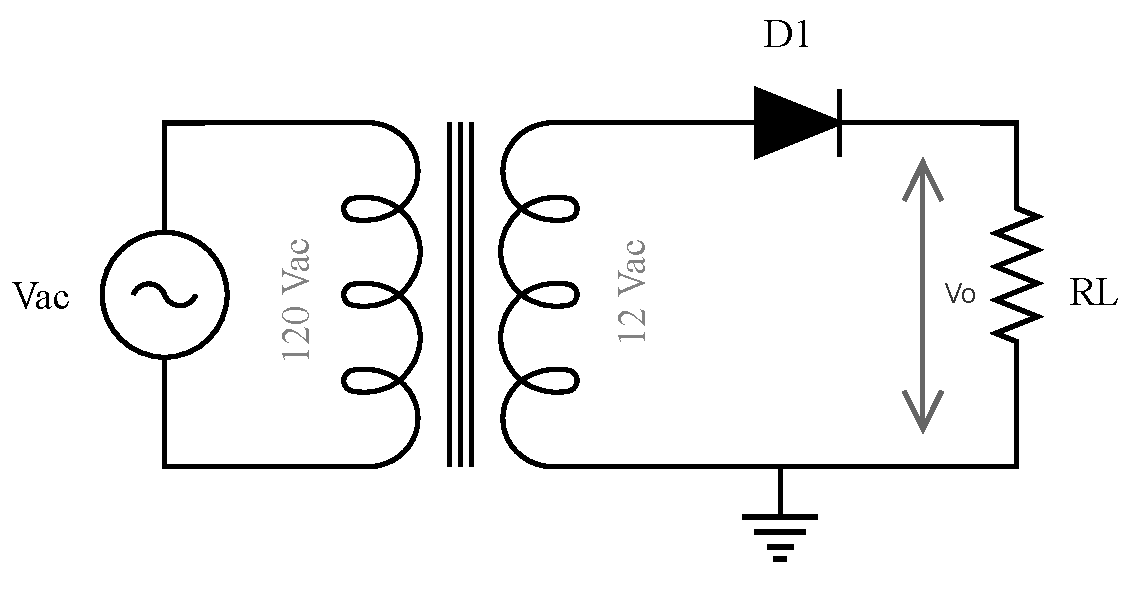
\includegraphics[scale=0.45]{RMO}    %Comando para agregar la imagen
\caption{Pie de imagen: Imagen con extensión PDF}  %Agregar pie de texto
\label{Fig:Rectificador}         %Etiqueta de la imagen           
\end{figure}  

\begin{figure}[h!] \centering
\includegraphics[scale=0.05]{BUTTON}
\caption{Pie de imagen: Fotografía con extensión  JPG}
\label{Fig:PushButton}
\end{figure}  


Para referenciar o nombrar una figura en el texto utilizamos el comando ref seguido de la etiqueta de la figura, tal y como se observa en el siguiente ejemplo: 

\textit{En la Figura \ref{Fig:Rectificador} se muestra el circuito esquemático del  rectificador de media onda mientras que  en la Figura \ref{Fig:PushButton} se muestra un circuito básico en protoboard.}


%%%%%%%%%%%%%%%%%%%%%%%%%%%%%%%
%%%%%%%%% ECUACIONES %%%%%%%%%%
%%%%%%%%%%%%%%%%%%%%%%%%%%%%%%%
\subsection{Ecuaciones en \LaTeX}

Para escribir una ecuación utilizamos los siguientes comandos:
\begin{equation}
\label{eqID}        %Etiqueta de la ecuacion
I_D=\frac{q N_A n_i^2}{N_D}\left(\frac{\alpha V_{GS}^2}{\mu_o}\right)^3
\end{equation}

\begin{equation}\label{Voeq} 
V_o \approx \int e^XdX
\end{equation}

Para referenciar o nombrar una ecuación en el texto utilizamos los mismos comandos que se utilizaron para referenciar imagenes tal y como se observa en el siguiente ejemplo:

Las ecuaciones (\ref{eqID} y (\ref{Voeq}) muestran las formulas para calcular $I_D$ y $V_o$ respectivamente.

En el ejemplo anterior se observo tambien que se pueden añadir simbolos matemáticos e incluso ecuaciones sencillas simplemente encerrando las expresiones entre los símbolos de pesos. Por ejemplo: $\alpha$, $I_2$, $I=V/R$. 

Se pueden reportar despejes, cálculos, procedimientos y formulas sin enumerarlos. Por ejemplo el siguiente cálculo:
\begin{gather*}
i=\frac{v}{R}\Longrightarrow i=\frac{5}{500}=10 mA
\end{gather*}
%%%%%%%%%%%%%%%%%%%%%%%%%%%%%%%
Una manera sencilla de generar el código para escribir ecuaciones es utilizando la página \url{http://www.hostmath.com/}
%%%%%%%%%%%%%%%%%%%%%%%%%%%
%%%%%%%%% TABLAS %%%%%%%%%%
%%%%%%%%%%%%%%%%%%%%%%%%%%%
\subsection{Tablas en \LaTeX}
Para definir una tabla se utilizan los siguientes comandos:

\begin{table}[h!] \centering
%%%%%%%%%  El siguiente codigo genera la tabla
\begin{tabular}{@{}|c|l|l|l|@{}}
\hline
\multicolumn{1}{|l|}{\textbf{$f (Hz)$}} & \textbf{$v_o$} & \textbf{$G$} & \textbf{$G_{calc}$}\\ \hline
100                                                         &             &         &    \\ \hline
200                                                       &             &           &  \\ \hline
400                                                       &             &            & \\ \hline
800                                                       &             &           &  \\ \hline
1600                                                      &             &           &  \\ \hline
\end{tabular}
%%%%%%%%%%%%%%%%%%%%%%%%%%%%%%%%%%%%%%%
% El siguiente codigo es el pie de tabla
\caption{Variación de frecuencia en el derivador}
%El siguiente codigo es la etiqueta de la tabla
\label{Tab:P2_DERFREQ}
\end{table}   

Para referenciar tablas lo hacemos de la misma forma que se hizo con las imágenes y ecuaciones. Por ejemplo: En la tabla \ref{Tab:P2_DERFREQ} se anotaran los resultados de la variación de frecuencia de la señal de entrada del circuito derivador.

Una manera sencilla de generar el código para escribir ecuaciones es utilizando la página \url{https://www.tablesgenerator.com/}

%%%%%%%%%%%%%%%%%%%%%%%%%%%%%%
%%%%% CITAR BIBLIOGRAFIA %%%%%
%%%%%%%%%%%%%%%%%%%%%%%%%%%%%%
\subsection{Citar en formato IEEE}
Para citar referencias bibliográficas se usa el comando cite seguido de la etiqueta de la referencia previamente agregada en la bibliografía. A continuacion se muestran algunos ejemplos:

En \cite{nombre_para_citar} se muestran los campos que deben llenarse en una referencia, en \cite{kopka} se muestra un ejemplo, y en \cite{link} se muestra como citar un enlace. Preferiblemente citar libros y artículos.

%%%%%%%%%


